% !TeX root = ../main.tex
% Add the above to each chapter to make compiling the PDF easier in some editors.

\chapter{Skin- and Blood-Light Interaction}\label{chapter:Skin- and Blood-Light Interaction}

\section{Skin-Light Interaction}

The relationship between an optical radiation and human skin depends
on the absorption and scattering properties of three skin layers, listing from the outside: epidermis, dermis, and hypodermis \parencite{skin}.
 
The structures and component chromophores of these layers determine the behaviour of radiation. Understanding the penetration of optical radiation can be achieved by studying and analyzing the wavelength-dependent interactions of light with skin. For example, melanin exhibits maximum absorption in the UV and blue spectral
ranges, whereas blood absorbs blue and yellow light. The chromophores, such as melanin, blood, water, and lipid determine skin absorption \parencite{skin1}.
We will focus on the epidermis and dermis as the blood vessels are contained in the dermis

\subsubsection{Absorption and Scattering Properties of Epidermis and Dermis in the NIR Spectrum}

As the outermost skin layer, the epidermis forms the actual protective covering against environmental influences. The average thickness of epidermis is approximately 0.1 mm. However, on the face it maybe as thin as 0.02 mm, while on the soles of the feet it is as thick as 1–5 mm. Absorption and scattering of epidermis in the visible and NIR spectral ranges are defined almost exclusively by its melanin, the protein that adds pigment to skin, and water contents, respectively \parencite{skin1}.

The next layer is dermis, it is composed of gel-like and elastic materials, water, and, primarily, collagen. Embedded in this layer are systems and structures like lymph channels, blood vessels, nerve fibres, and muscle cells. Blood and water content define the absorptive properties of dermis in the visible and NIR range\parencite{skin1}.

Absorption and scattering coefficients of skin layers are shown in figures below \parencite{skin1}. The graphs demonstrate that the scattering of skin layers decreases with the increasing wavelength. 


\begin{figure}[H]
\centering
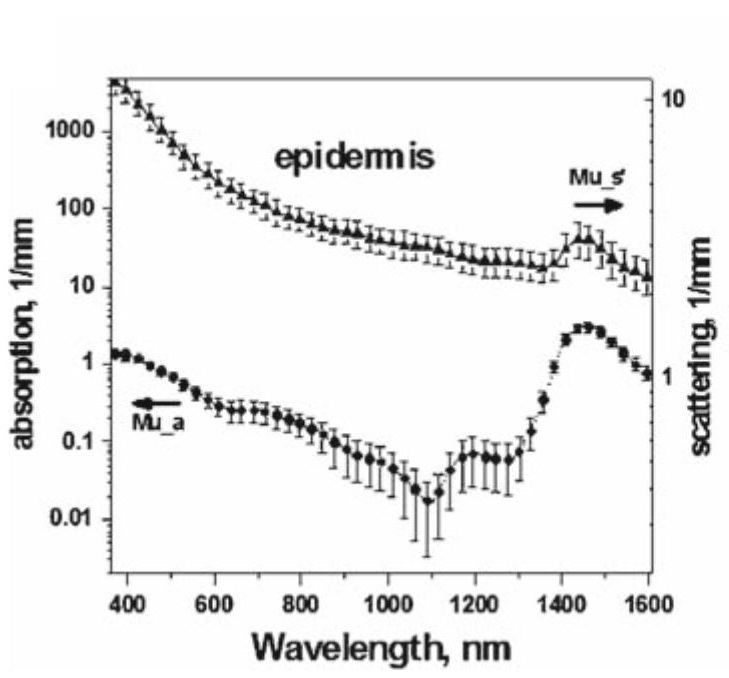
\includegraphics[scale=0.5]{figures/epidermis.JPG}
\caption[Optical properties of epidermis]{Optical properties of epidermis, Triangles – reduced scattering coefficients, circles absorption coefficients, bars – standard errors. Averaged over 7 samples.}\label{fig:epidermis}
\end{figure}





\begin{figure}[H]
\centering
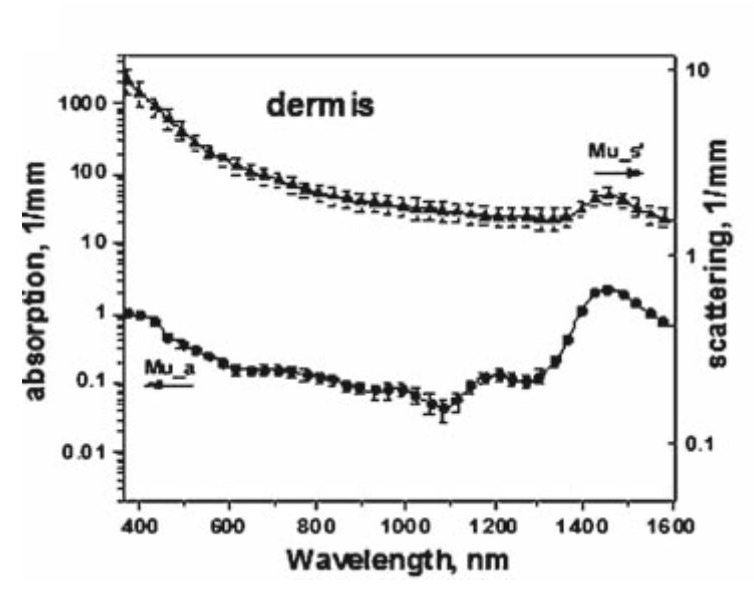
\includegraphics[scale=0.5]{figures/dermis.JPG}
\caption[Optical properties of dermis]{Optical properties of dermis. Triangles – reduced scattering coefficients,  circles absorption coefficients, bars – standard errors. Averaged over 8 samples.}\label{fig:dermis}
\end{figure}


\section{Blood-Light Interaction}


The optical properties of human blood under normal physiological conditions are largely determined by light interactions with plasma and red blood cells \parencite{opticsOfBlood}, which account for 99\% of the cellular elements \parencite{opticsOfBlood1}. 
The effects of the optical properties of WBCs and platelets on the light scattering and absorption by whole blood are considered negligible \parencite{opticsOfBlood}.

\subsubsection{Absorption and Scattering Properties of Red Blood Cells in the NIR Spectrum}
Red blood cells have a thin plasma membrane that encloses mainly a hemoglobin solution. The absorption and scattering of light by the RBCs are two to three orders of magnitude higher than those of the other blood components \parencite{opticsOfBlood1}. The light scattered by a single RBC depends on
its shape, volume, refractive index and orientation \parencite{opticsOfBlood1}. However the absorption of light by the RBCs is dominated by hemoglobin in its functional, oxygen-binding, forms, namely oxyhemoglobin and deoxyhemoglobin. 

\section{Conclusion: Wavelength Selection}
to quantify the absorption of light traveling within this solution [69]. It is necessary to take into account, however, that the optical path of
light traveling within a cell may increase due to multiple reflections at its internal boundary [